\section{Lower bounds on the distance-two support}\label{sec:bounds}

\subsection{Distance-two relaxations}\label{sec:relax}

\begin{lemma}\label{lem:half}
Let $\mathcal C$ be an optimal clustering, $S\in\mathcal C$ and $v\in S$.  Then
$|N(v)\cap S|\ge (|S|-1)/2$.  Consequently any two vertices of $S$ are
adjacent or have a common neighbour in $S$.  In particular every pair at
distance at least three is separated.
\end{lemma}
\begin{proof}
Moving $v$ to a singleton changes the cost by $|N(v)\cap S|-(|S|-1-|N(v)\cap
S|)$, which must be non-negative.  For non-adjacent $u,v\in S$ the sets
$N(u)\cap S$ and $N(v)\cap S$ lie in $S\setminus\{u,v\}$, which has $|S|-2$
elements, and have total size at least $|S|-1$, so they intersect.
\end{proof}

Lemma~\ref{lem:half} is folklore; its consequence for distance-three pairs is
noted by \citet{BastosOPSMP16} and used to forbid pairs in the
branch-and-bound of \citet{BlasiusEtAl22sea}.  What follows uses it to
restrict the LP rather than the search.

Let $\Nt=\{uv\notin\Ep: N(u)\cap N(v)\ne\emptyset\}$, $P=\Ep\cup\Nt$ and
$F=\binom V2\setminus P$ (the \emph{far} pairs).  Note
$|P|\le m+\sum_{w}\binom{\deg(w)}{2}$.  Figure~\ref{fig:support} shows
the support on a small neighbourhood of a collaboration network: already
there, 587 of the 780 pairs (75\%) are far and disappear from the relaxation.

\begin{figure}[!tbp]
\centering
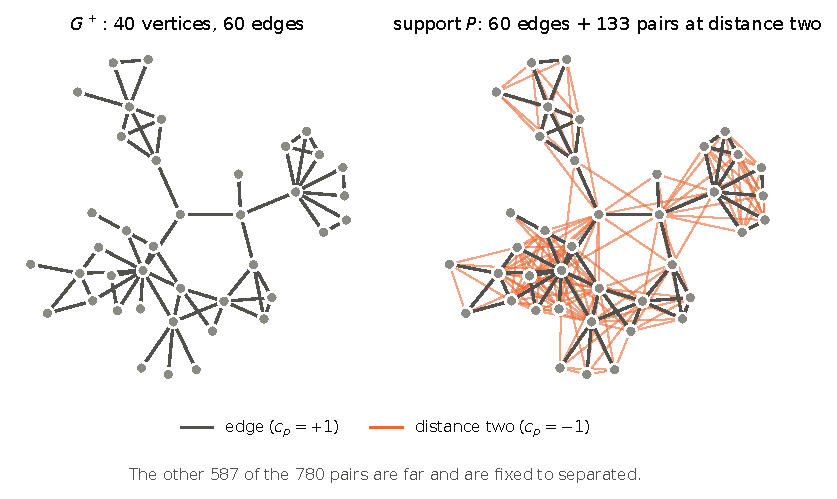
\includegraphics[width=0.9\textwidth]{figures/fig_support.pdf}
\caption{The distance-two support on a 40-vertex neighbourhood of
\texttt{ca-GrQc}.  Left: the positive graph.  Right: the support $P$ adds the
non-adjacent pairs with a common neighbour (orange); every other pair is far,
separated in every optimal clustering (Lemma~\ref{lem:half}), and carries no
variable.}\label{fig:support}
\end{figure}

\begin{definition}[distance-two relaxation]
$\mathrm{LP}_P$ has a variable $x_e\in[0,1]$ for every $e\in P$ and minimises
$\sum_{e\in\Ep}x_e+\sum_{e\in\Nt}(1-x_e)$ subject to
\begin{align}
x_{uv}&\le x_{uw}+x_{wv} &&\text{for all } u,v,w \text{ with } uv,uw,wv\in P,\label{eq:t1}\\
x_{uw}+x_{wv}&\ge 1 &&\text{for all } u,v,w \text{ with } uw,wv\in P,\ uv\in F.\label{eq:t2}
\end{align}
\end{definition}

\begin{theorem}\label{thm:sparse}
Let $\mathrm{LP}_{\mathrm{std}}$ denote the value of the metric LP.
\begin{enumerate}
\item[(a)] $\mathrm{LP}_{\mathrm{std}}\le \mathrm{LP}_P\le\OPT$.
\item[(b)] If $x$ is feasible for $\mathrm{LP}_P$, then $\bar x$, defined as $x$ on
$P$ and $1$ on $F$, is feasible for the metric LP and has the same cost.
\item[(c)] Let $\mathcal A$ be a randomised rounding algorithm with
$\mathbb E[\cost(\mathcal A(\bar x))]\le\alpha\,\mathrm{cost}(\bar x)$ for every
feasible metric $\bar x$.  Applied to an optimal solution of $\mathrm{LP}_P$ it
is an $\alpha$-approximation.  This holds in particular for $\alpha=2.5$
(ACN) and $\alpha=2.06$ (CMSY).  With pivot-based rounding, only pairs in
$P$ can be joined, so the rounding takes $O(n+|P|)$ time.
\end{enumerate}
\end{theorem}
\begin{proof}
(b) Consider a triple $u,v,w$ and the number of far pairs among $uv,uw,wv$.
With none, all three triangle inequalities are rows~\eqref{eq:t1}.  With
exactly one, say $uv$, the inequality $\bar x_{uv}=1\le x_{uw}+x_{wv}$ is
row~\eqref{eq:t2}.  The other two inequalities, such as
$x_{uw}\le 1+x_{wv}$, hold because $x\le 1$.  With two or three far pairs, each
inequality has a right-hand side of at least $1$.  Far pairs are negative and
$\bar x=1$ on them, so they contribute $0$ to the cost.  (a) The first
inequality follows from (b).  For the second, by Lemma~\ref{lem:half} an
optimal clustering separates all far pairs.  Its cut vector restricted to $P$
therefore satisfies~\eqref{eq:t1} and~\eqref{eq:t2}, because it is a metric
with $x=1$ on $F$, and it has cost $\OPT$.  (c) follows from (a) and (b): the
expected cost is at most $\alpha\,\mathrm{cost}(\bar x)=\alpha\,\mathrm{LP}_P
\le\alpha\,\OPT$.  Pivot-based rounding joins $v$ to the pivot $u$ with
probability $1-f(x_{uv})$, and $f(1)=1$ for both rounding functions.
\end{proof}

The rows~\eqref{eq:t1}--\eqref{eq:t2} are generated lazily.  A violated row
needs $x_{uw}+x_{wv}<1$, so separation around a vertex $w$ only has to look at
pairs of ``close'' neighbours in $P$, which keeps it fast in practice.

\paragraph{Stronger inequalities.}  The integrality gap of the metric LP is
at least $2$ (stars attain it asymptotically) and at most
$2.06$~\citep{ChawlaMSY15}.  We add two families that are valid for every clustering
separating all far pairs, and hence for every optimal clustering.

\begin{proposition}\label{prop:subgraph}
Let $\mathcal C$ be a clustering in which no far pair shares a cluster.
\begin{enumerate}
\item[(i)] (star inequalities; the case $|S|=1$ of the $2$-partition
inequalities of \citet{GrotschelW89}) For every $v$ and $T\subseteq V\setminus\{v\}$, with
$y=1-x^{\mathcal C}$,
\[\textstyle\sum_{t\in T}y_{vt}-\sum_{\{t,t'\}\subseteq T,\ tt'\in P}y_{tt'}\le 1.\]
\item[(ii)] (local subgraph inequalities) For every $H\subseteq V$,
\[\textstyle\sum_{e\in\Ep(H)}x^{\mathcal C}_e+\sum_{e\in\Nt(H)}(1-x^{\mathcal C}_e)\ \ge\ \OPT(H),\]
where $\OPT(H)$ is the optimum of the instance induced by $H$ and $\Ep(H)$,
$\Nt(H)$ are the pairs of $\Ep$ and $\Nt$ inside $H$.
\end{enumerate}
\end{proposition}
\begin{proof}
(i) If the cluster of $v$ contains $k$ vertices of $T$, the first sum is $k$
and the second is at least $\binom k2$.  Pairs inside $T$ that are not in $P$
are far, so they are separated and contribute $0$ to the second sum.
Finally $k-\binom k2\le1$.  (ii) Restricted to $H$, $\mathcal C$ is a clustering
of $H$.  Its mistakes inside $H$ number at least $\OPT(H)$.  The far pairs
inside $H$ are separated and cost nothing, so all its mistakes are counted
on the left-hand side.
\end{proof}

The local subgraph inequalities are local cuts in the sense of
\citet{ApplegateBCC01localcuts}: valid inequalities obtained by solving a small
subproblem exactly.  Bad triangles ($\OPT=1$) and induced stars with $k$ independent leaves
($\OPT=k-1$) are local subgraph inequalities.  So are chordless cycles $C_k$,
for which $\OPT(C_k)=\lceil k/2\rceil$ while the metric LP only certifies
$k/2$ (put $x=1/2$ on the cycle edges).  We separate stars greedily around
each vertex.  For (ii) we grow $H$ ($|H|\le 8$) by breadth-first search along
fractional pairs and compute $\OPT(H)$ by enumerating the at most $4140$
set partitions of $H$.

\subsection{Anytime dual bounds}\label{sec:dual}

Write the relaxation as $\min\{K+c^\top x: Ax\ge b,\ 0\le x\le 1\}$ over
$x\in\R^P$, with $c_e=1$ on $\Ep$, $c_e=-1$ on $\Nt$ and $K=|\Nt|$.  The rows
of $(A,b)$ are any valid inequalities from Section~\ref{sec:relax}.

\begin{theorem}\label{thm:anytime}
For every $y\ge 0$ let $r=c-A^\top y$ and
\begin{equation}\label{eq:lb}
\LB(y)=K+b^\top y+\sum_{e\in P}\min\{0,r_e\}.
\end{equation}
\begin{enumerate}
\item[(a)] $\LB(y)\le\OPT$.
\item[(b)] Let $B\subseteq V$, let $R_B$ be a set of rows supported on pairs
with both endpoints in $B$, and let $\bar r$ be the reduced costs after
removing the contribution of the current multipliers on $R_B$.  Replace these
multipliers by an optimal dual solution of
$\min\{\bar r^\top x_B: A_Bx_B\ge b_B,\ 0\le x_B\le 1\}$.  This does not
decrease $\LB$.
\item[(c)] If $B=V$ and $R_B$ contains all rows of $\mathrm{LP}_P$, one block
step gives $\LB=\mathrm{LP}_P$.
\end{enumerate}
\end{theorem}
\begin{proof}
(a) Let $\mathcal C$ be optimal.  By Lemma~\ref{lem:half} it separates far
pairs, so $\OPT=K+c^\top x^{\mathcal C}$ with $x^{\mathcal C}\in\{0,1\}^P$
satisfying $Ax^{\mathcal C}\ge b$.  Then
$\OPT=K+r^\top x^{\mathcal C}+y^\top Ax^{\mathcal C}\ge K+\sum_e\min\{0,r_e\}+y^\top b$.
(b) By LP duality the block LP equals
$\max_{y_B\ge0}\ b_B^\top y_B+\sum_{e\in P_B}\min\{0,(\bar r-A_B^\top
y_B)_e\}$.  The terms of~\eqref{eq:lb} outside the block do not change, and
the old multipliers are feasible for this maximisation.  (c) is LP duality
for $\mathrm{LP}_P$ with the box constraints.
\end{proof}

Part~(b) needs an optimal block dual.  When a block LP stops at its time limit,
its duals are only feasible; the bound computed with them is still valid by
part~(a), but it may be smaller than before.  The implementation therefore
evaluates the new bound and keeps a block step only if the bound does not
decrease, so the bound is monotone in every case.

\paragraph{Warm start by star packings.}  Every pair-disjoint family of
induced stars (a centre $v$ with $k\ge2$ pairwise non-adjacent positive
neighbours) is a feasible dual solution: put $y=1$ on the corresponding
local subgraph inequalities of Proposition~\ref{prop:subgraph}(ii), which in
$x$-form read $\sum_t x_{vt}-\sum_{tt'}x_{tt'}\ge (k-1)-\binom k2$.  Then
$\LB(y)$ equals the packing value $\sum(k-1)$.  Indeed, a centre pair has
$c_e=1$ and coefficient $1$, and a leaf pair has $c_e=-1$ and coefficient
$-1$, so every packed pair has reduced cost $0$.  Unpacked pairs keep
$r_e=c_e$.  Hence $\LB=K+\sum_S\big((k_S-1)-\binom{k_S}2\big)-|\Nt\setminus
\text{packed}|$, and $K-|\Nt\setminus\text{packed}|=\sum_S\binom{k_S}{2}$.
Fractional packings of bad triangles, as computed by the Garg--K\"onemann
scheme~\citep{GargK07,Fleischer00}, are installed in the same way on the
rows $x_{uw}+x_{wv}-x_{uv}\ge0$.
Packings are the bounds used inside the KaPoCE branch-and-bound
algorithm~\citep{BlasiusEtAl22sea}.  Its implementation stores the instance
as a dense matrix, so it applies only to graphs with at most about $10^4$
vertices.  We build a greedy packing on the sparse support, processing
centres by decreasing degree, and improve it by \emph{ruin and recreate}.
(On dense instances large stars waste pairs, since a star with $k$ leaves
uses $k+\binom k2$ pairs for a value of $k-1$.  There we also try a packing
that first packs bad triangles maximally and then extends stars on free
pairs, as well as the fractional triangle packing, and install the best of
the candidates.)
Each step picks a random vertex, removes all stars centred in a random
connected region of about 12 vertices around it, and repacks the freed
pairs greedily in a random order.  A step is kept iff the value does not
decrease.  The packing is installed as the initial multipliers.  Subsequent
block steps release the packed rows that lie inside a block and re-optimise
them fractionally together with newly separated rows.  By
Theorem~\ref{thm:anytime}(b), the final bound is never below the packing
value.

The bound~\eqref{eq:lb} needs only the vector $r$ and the scalar $b^\top y$.
We store the rows with positive multipliers so that a later block containing
them can re-optimise them.  Blocks of the same partition are independent.
In a \emph{sweep} we compute a partition into parts of about $2500$ vertices
with METIS~\citep{KarypisK98} on a randomly relabelled copy of $G^+$, so that
successive sweeps cut different pairs.  Each part is solved with the dual
simplex method of HiGHS~\citep{HuangfuH18}, with lazily separated triangle,
star and local subgraph rows.  After the sweeps stall we switch to
\emph{gap-guided blocks}, grown around the vertices with the largest share of
the gap defined next.  Because~\eqref{eq:lb} is valid for any $y\ge0$, the
bound remains correct even when a block LP hits its time limit.  We only
clamp the dual values to be non-negative, and reject a block step that would
lower the bound.

\paragraph{Floating point.}  The block LPs are solved in double precision,
so the multipliers $y$ are inexact and the rows they carry are generated by
floating-point separation.  Neither affects validity: \eqref{eq:lb} holds for
every $y\ge0$ and every set of valid rows.  The value the solver reports is
nevertheless not the value we publish.  Section~\ref{sec:cert} recomputes it
from the exported rows and multipliers in exact arithmetic, after checking
every row, and all bounds in Section~\ref{sec:exp} are these recomputed
values.

